\documentclass[a4paper,12pt]{article}
\usepackage[a4paper,top=1.3cm,bottom=2cm,left=1.5cm,right=1.5cm,marginparwidth=0.75cm]{geometry}
\usepackage{cmap}
\usepackage{mathtext}
\usepackage[T2A]{fontenc}
\usepackage[utf8]{inputenc}
\usepackage[english,russian]{babel}
\usepackage{siunitx}
\usepackage{enumitem}
\usepackage{placeins}

\usepackage{graphicx}
\usepackage{subcaption}
\usepackage{amsmath}

\usepackage{wrapfig}
\usepackage{tabularx}
\usepackage{multirow}

\usepackage{hyperref}
\usepackage[rgb]{xcolor}
\hypersetup{colorlinks=true,urlcolor=blue}
\usepackage{siunitx}
\usepackage{amsmath,amsfonts,amssymb,amsthm,mathtools}
\usepackage{mathtools}
\usepackage{icomma}
\mathtoolsset{showonlyrefs=false}
\usepackage{euscript}
\usepackage{mathrsfs}
\DeclareMathOperator{\sgn}{\mathop{sgn}}
\newcommand*{\hm}[1]{#1\nobreak\discretionary{}
{\hbox{$\mathsurround=0pt #1$}}{}}

\newcommand\labname{Определение ширины запрещённой зоны полупроводника}
\newcommand\labnumber{11.1}

\author{Макаров Лев Евгеньевич}
\title{Лабораторная работа №\labnumber\\\labname}
\date{\today}

\makeatletter
\AddEnumerateCounter{\asbuk}{\russian@asbuk@alph}{щ}
\makeatother

\begin{document}

\begin{titlepage}
    \begin{center}
        {\large МОСКОВСКИЙ ФИЗИКО-ТЕХНИЧЕСКИЙ ИНСТИТУТ (НАЦИОНАЛЬНЫЙ ИССЛЕДОВАТЕЛЬСКИЙ УНИВЕРСИТЕТ)}
    \end{center}
    \begin{center}
        {\large Физтех-школа фотоники, электроники и молекулярной физики}
    \end{center}

    \vspace{4.5cm}
    {\huge
        \begin{center}
            {\bf Отчёт о выполнении лабораторной работы \labnumber}\\
            \labname
        \end{center}
    }
    \vspace{2cm}
    \begin{flushright}
        {\LARGE Автор:\\ Макаров Лев Евгеньевич\\
        \vspace{0.2cm}
        Б04-306}
    \end{flushright}
    \vspace{8cm}
    \begin{center}
        Долгопрудный 2026
    \end{center}
\end{titlepage}

\section{Введение}

\textbf{Цель работы:}
\begin{enumerate}
    \item исследовать температурную зависимость электропроводности полупроводника с помощью моста переменного тока;
    \item построить зависимости $\sigma(T)$ и $\ln \sigma(1/T)$;
    \item определить ширину запрещённой зоны исследуемого полупроводника по наклону графика $\ln \sigma(1/T)$.
\end{enumerate}

\textbf{В работе используются:} мост переменного тока, генератор звуковой частоты, осциллограф, нагревательная печь, медь--константановая термопара, цифровой вольтметр, магазин сопротивлений.

\section{Теоретические сведения}

В собственном полупроводнике электроны переходят из валентной зоны в зону проводимости за счёт теплового возбуждения. Если ширина запрещённой зоны равна $\Delta$, то концентрация носителей заряда имеет экспоненциальную зависимость от температуры:

\begin{equation}
    n \propto \exp \left( -\frac{\Delta}{2k_{\text{Б}}T} \right).
\end{equation}

Электропроводность полупроводника пропорциональна концентрации носителей, поэтому

\begin{equation}
    \sigma = A \exp \left( -\frac{\Delta}{2k_{\text{Б}}T} \right),
    \label{eq:sigma-theory}
\end{equation}

где слабая температурная зависимость предэкспоненциального множителя не учитывается. Логарифмируя \eqref{eq:sigma-theory}, получаем

\begin{equation}
    \ln \sigma = B + C \frac{1}{T}, \qquad C = -\frac{\Delta}{2k_{\text{Б}}}.
    \label{eq:linear}
\end{equation}

Отсюда ширина запрещённой зоны определяется по наклону прямой:

\begin{equation}
    \Delta = -2k_{\text{Б}} C.
    \label{eq:delta}
\end{equation}

\section{Экспериментальная установка}

В работе была выполнена часть с измерением температурной зависимости электропроводности на мосте переменного тока. Исследуемый полупроводниковый образец является одним из плеч моста. Остальные плечи образованы сопротивлениями $R_1$, $R_2$, $R_3$, причём $R_2$ --- магазин сопротивлений, которым достигается баланс моста.

При балансе моста сопротивление образца выражается через сопротивления плеч:

\begin{equation}
    R_x = \frac{R_3}{R_1} R_2.
\end{equation}

Для образца длиной $l$ и площади поперечного сечения $S$ удельная электропроводность равна

\begin{equation}
    \sigma = \frac{l}{R_x S} = \frac{lR_1}{SR_3R_2}.
\end{equation}

В используемой схеме в обработке приняты

\begin{equation}
    R_1 = (220 \pm 0.5)~\text{Ом}, \qquad
    R_3 = (560 \pm 0.5)~\text{Ом}.
\end{equation}

Размеры полупроводникового образца:

\begin{equation}
    a = (40.0 \pm 0.5)~\text{мм}, \qquad
    b = (4.10 \pm 0.05)~\text{мм}, \qquad
    c = (4.150 \pm 0.005)~\text{мм}.
\end{equation}

Здесь $l = a$, $S = bc$. Температура измерялась медь--константановой термопарой, ЭДС которой регистрировалась цифровым вольтметром.

\section{Результаты измерений и обработка данных}

\subsection*{Калибровка термопары}

Для пересчёта ЭДС термопары в температуру использовалась табличная калибровка. Зависимость температуры от ЭДС аппроксимировалась квадратичным многочленом

\begin{equation}
    t(\varepsilon) = a_0 + a_1 \varepsilon + a_2 \varepsilon^2,
    \label{eq:thermopair}
\end{equation}

где $\varepsilon$ измеряется в мкВ, а $t$ --- в $^\circ$C. Для коэффициентов получено

\begin{equation}
    a_0 = 0.16 \pm 0.05, \quad
    a_1 = (2.55 \pm 0.01)\cdot 10^{-2}, \quad
    a_2 = (-5.08 \pm 0.11)\cdot 10^{-7}.
\end{equation}

Погрешность температуры определялась по правилу распространения погрешностей:

\begin{equation}
    \sigma_t = \sqrt{ \sigma_{a_0}^2 + \varepsilon^2 \sigma_{a_1}^2 + \varepsilon^4 \sigma_{a_2}^2 + \left(a_1 + 2 \varepsilon a_2 \right)^2 \sigma_\varepsilon^2 }.
\end{equation}

Результат аппроксимации приведён на рис. \ref{pic:thermopair_approximation}.

\begin{figure}[h]
    \centering
    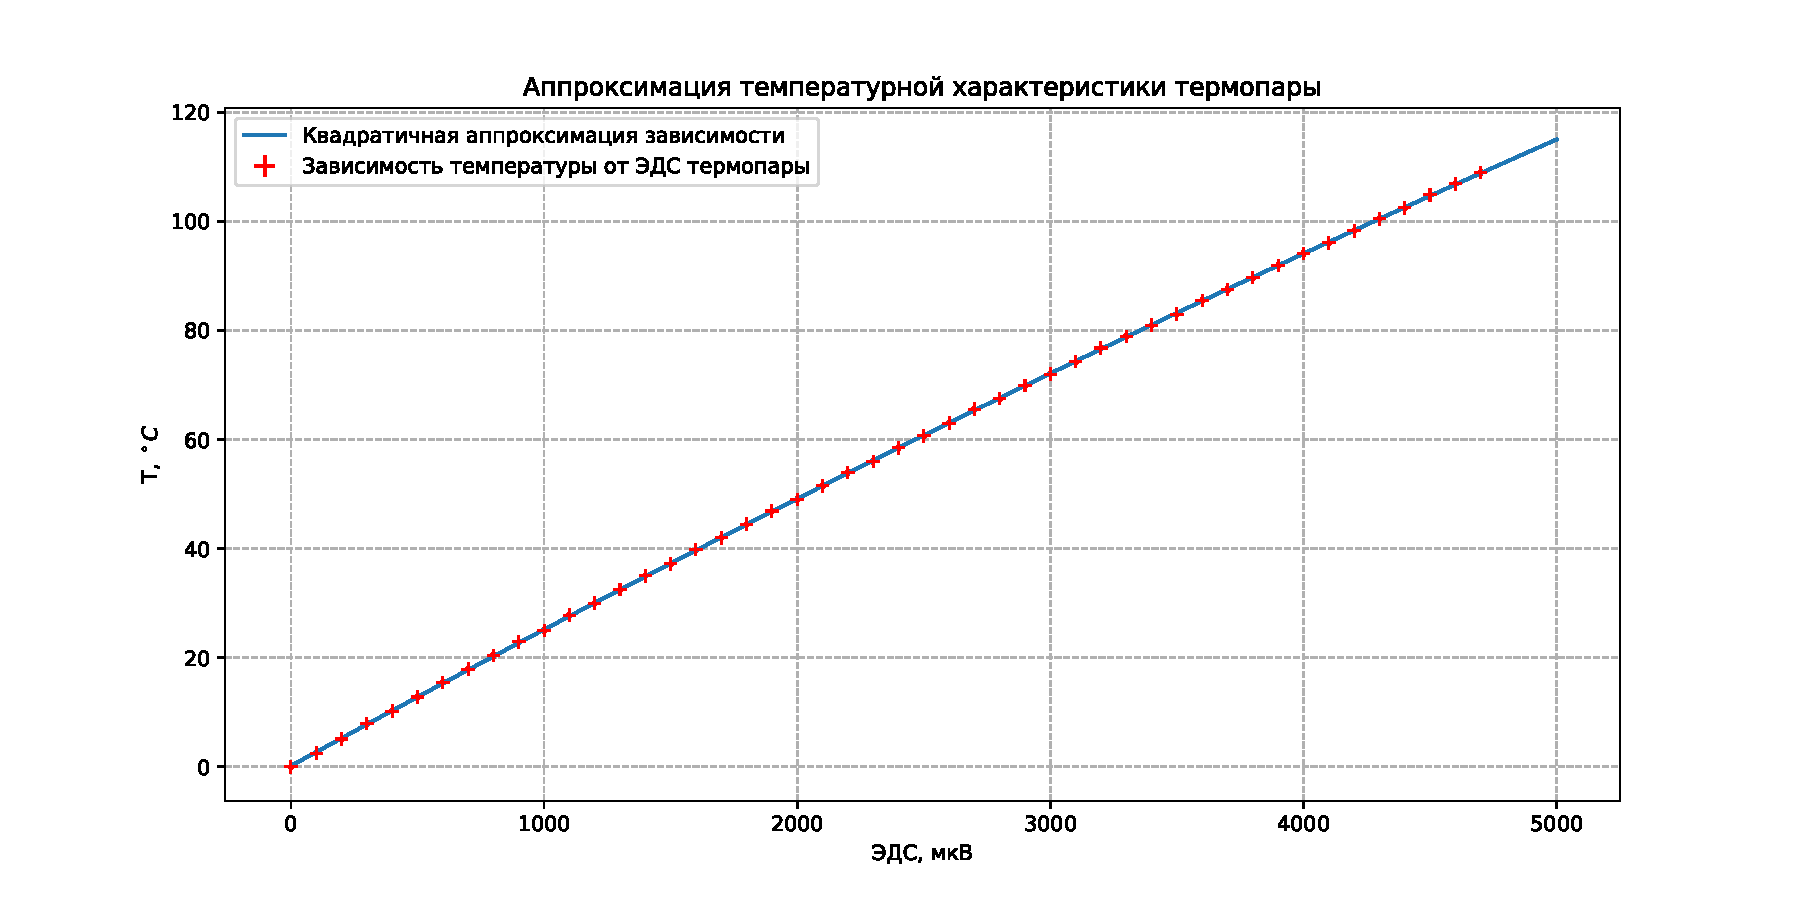
\includegraphics[width=0.9\textwidth]{pictures/thermopair_approximation.pdf}
    \caption{Аппроксимация температурной характеристики термопары}
    \label{pic:thermopair_approximation}
\end{figure}

\subsection*{Измерение электропроводности}

Нуль термопары соответствовал показанию $V_0 = -0.03~\text{мВ}$. Холодный спай находился при комнатной температуре

\begin{equation}
    t_0 = (24.5 \pm 0.5)~^\circ\text{C}.
\end{equation}

Результаты измерений и вычисленные значения электропроводности приведены в таблице \ref{tab:data}. В таблице $V$ --- показание вольтметра на термопаре, $R_2$ --- сопротивление магазина при балансе моста.

\begin{table}[h]
    \centering
    \small
    \caption{Измерение зависимости электропроводности от температуры}
    \label{tab:data}
    \begin{tabular}{|r|r|r|r|r|r|r|r|}
        \hline
        № & $R_2$, Ом & $V$, мВ & $t$, $^\circ$C & $T$, К & $\sigma$, $\text{Ом}^{-1}\text{м}^{-1}$ & $\ln\sigma$ & $10^3/T$, К$^{-1}$ \\
        \hline
         1 &  274.3 & -0.03 &  24.66 & 297.81 &       3.4 &  1.214 &  3.358 \\
         2 &  257.0 &  0.16 &  29.49 & 302.64 &       3.6 &  1.279 &  3.304 \\
         3 &  227.0 &  0.37 &  34.79 & 307.94 &       4.1 &  1.403 &  3.247 \\
         4 &  203.0 &  0.53 &  38.79 & 311.94 &       4.5 &  1.515 &  3.206 \\
         5 &  173.0 &  0.74 &  44.01 & 317.16 &       5.3 &  1.675 &  3.153 \\
         6 &  150.0 &  0.91 &  48.20 & 321.35 &       6.2 &  1.818 &  3.112 \\
         7 &  125.0 &  1.14 &  53.82 & 326.97 &       7.4 &  2.000 &  3.058 \\
         8 &  101.0 &  1.38 &  59.63 & 332.78 &       9.1 &  2.213 &  3.005 \\
         9 &   85.0 &  1.59 &  64.67 & 337.82 &      10.9 &  2.386 &  2.960 \\
        10 &   64.2 &  1.93 &  72.72 & 345.87 &      14.4 &  2.666 &  2.891 \\
        11 &   50.0 &  2.25 &  80.20 & 353.35 &      18.5 &  2.916 &  2.830 \\
        12 &   42.0 &  2.48 &  85.51 & 358.66 &      22.0 &  3.091 &  2.788 \\
        13 &   33.0 &  2.79 &  92.58 & 365.73 &      28.0 &  3.332 &  2.734 \\
        14 &   18.0 &  3.66 & 111.90 & 385.05 &      51.3 &  3.938 &  2.597 \\
        15 &   15.9 &  3.87 & 116.44 & 389.59 &      58.1 &  4.062 &  2.567 \\
        16 &    4.0 &  4.05 & 120.31 & 393.46 &     230.9 &  5.442 &  2.542 \\
        \hline
    \end{tabular}
\end{table}

Погрешность электропроводности рассчитывалась как

\begin{equation}
    \sigma_\sigma = \sigma \sqrt{
        \left(\frac{\sigma_l}{l}\right)^2 +
        \left(\frac{\sigma_{R_1}}{R_1}\right)^2 +
        \left(\frac{\sigma_{R_3}}{R_3}\right)^2 +
        \left(\frac{\sigma_S}{S}\right)^2 +
        \left(\frac{\sigma_{R_2}}{R_2}\right)^2
    }.
\end{equation}

Для логарифма электропроводности использовалась погрешность

\begin{equation}
    \sigma_{\ln \sigma} = \frac{\sigma_\sigma}{\sigma},
\end{equation}

а для обратной температуры:

\begin{equation}
    \sigma_{1/T} = \frac{\sigma_T}{T^2}.
\end{equation}

График зависимости $\sigma(T)$ приведён на рис. \ref{pic:sigma-T}.

\begin{figure}[h]
    \centering
    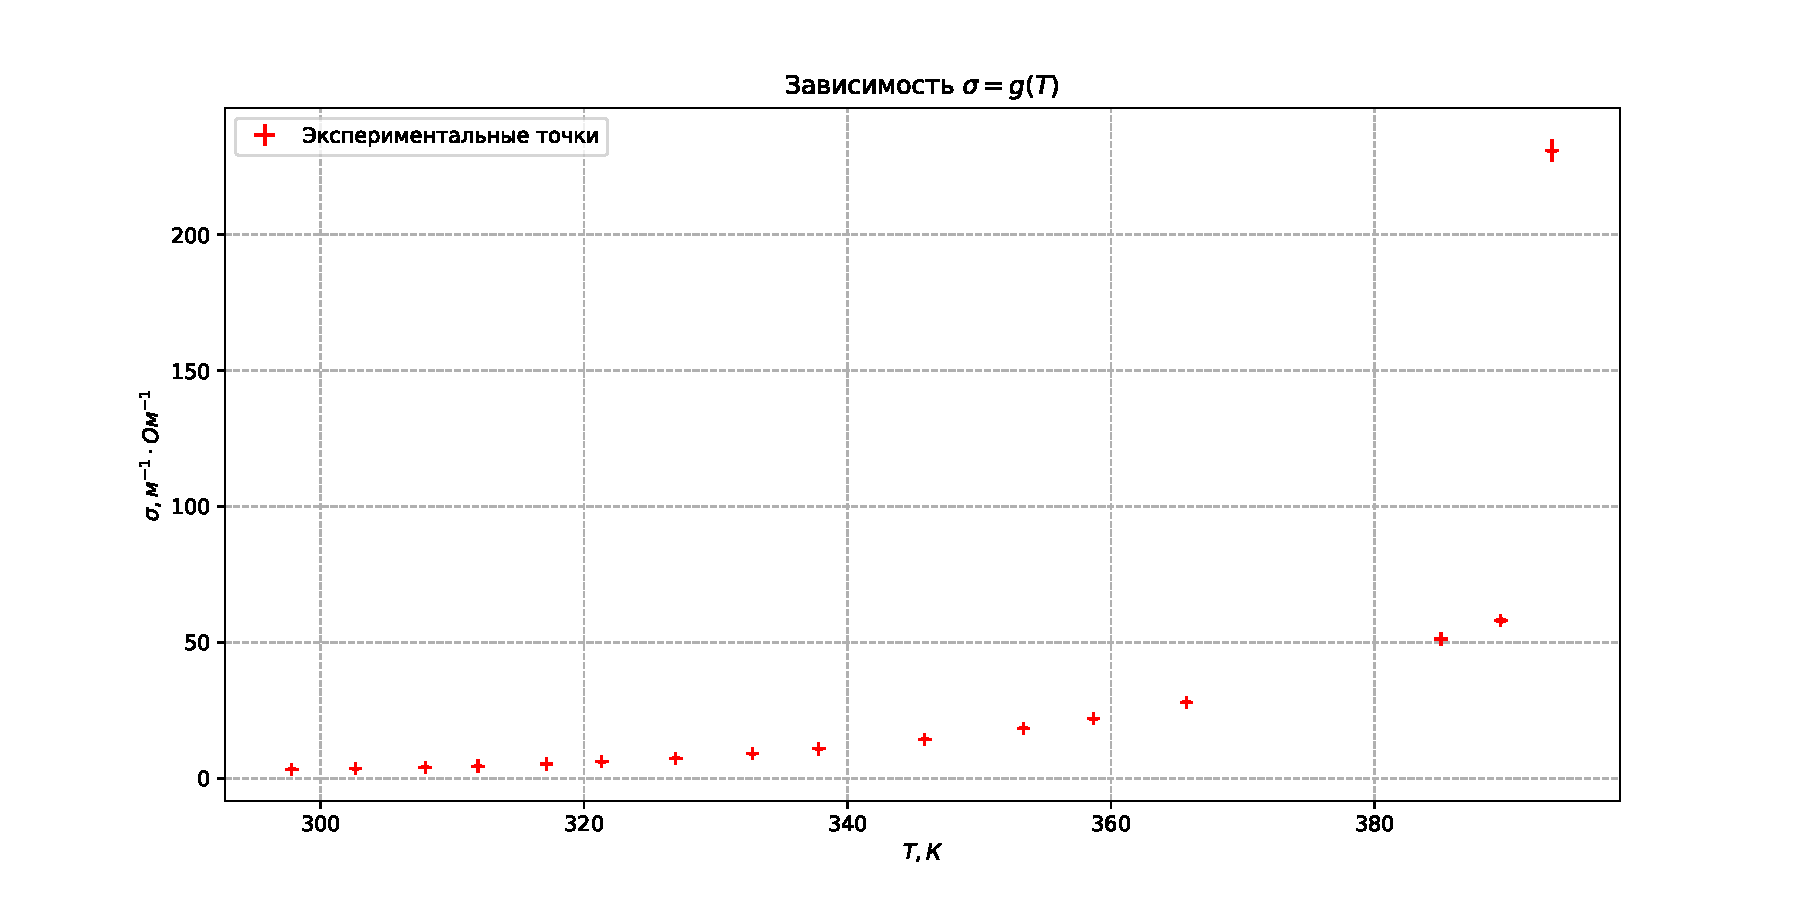
\includegraphics[width=0.9\textwidth]{pictures/sigma_T_graph.pdf}
    \caption{Зависимость электропроводности полупроводника от температуры}
    \label{pic:sigma-T}
\end{figure}

\subsection*{Определение ширины запрещённой зоны}

Построим зависимость $\ln \sigma$ от $1/T$ и аппроксимируем её прямой вида \eqref{eq:linear}. График приведён на рис. \ref{pic:ln-sigma-T}.

\begin{figure}[h]
    \centering
    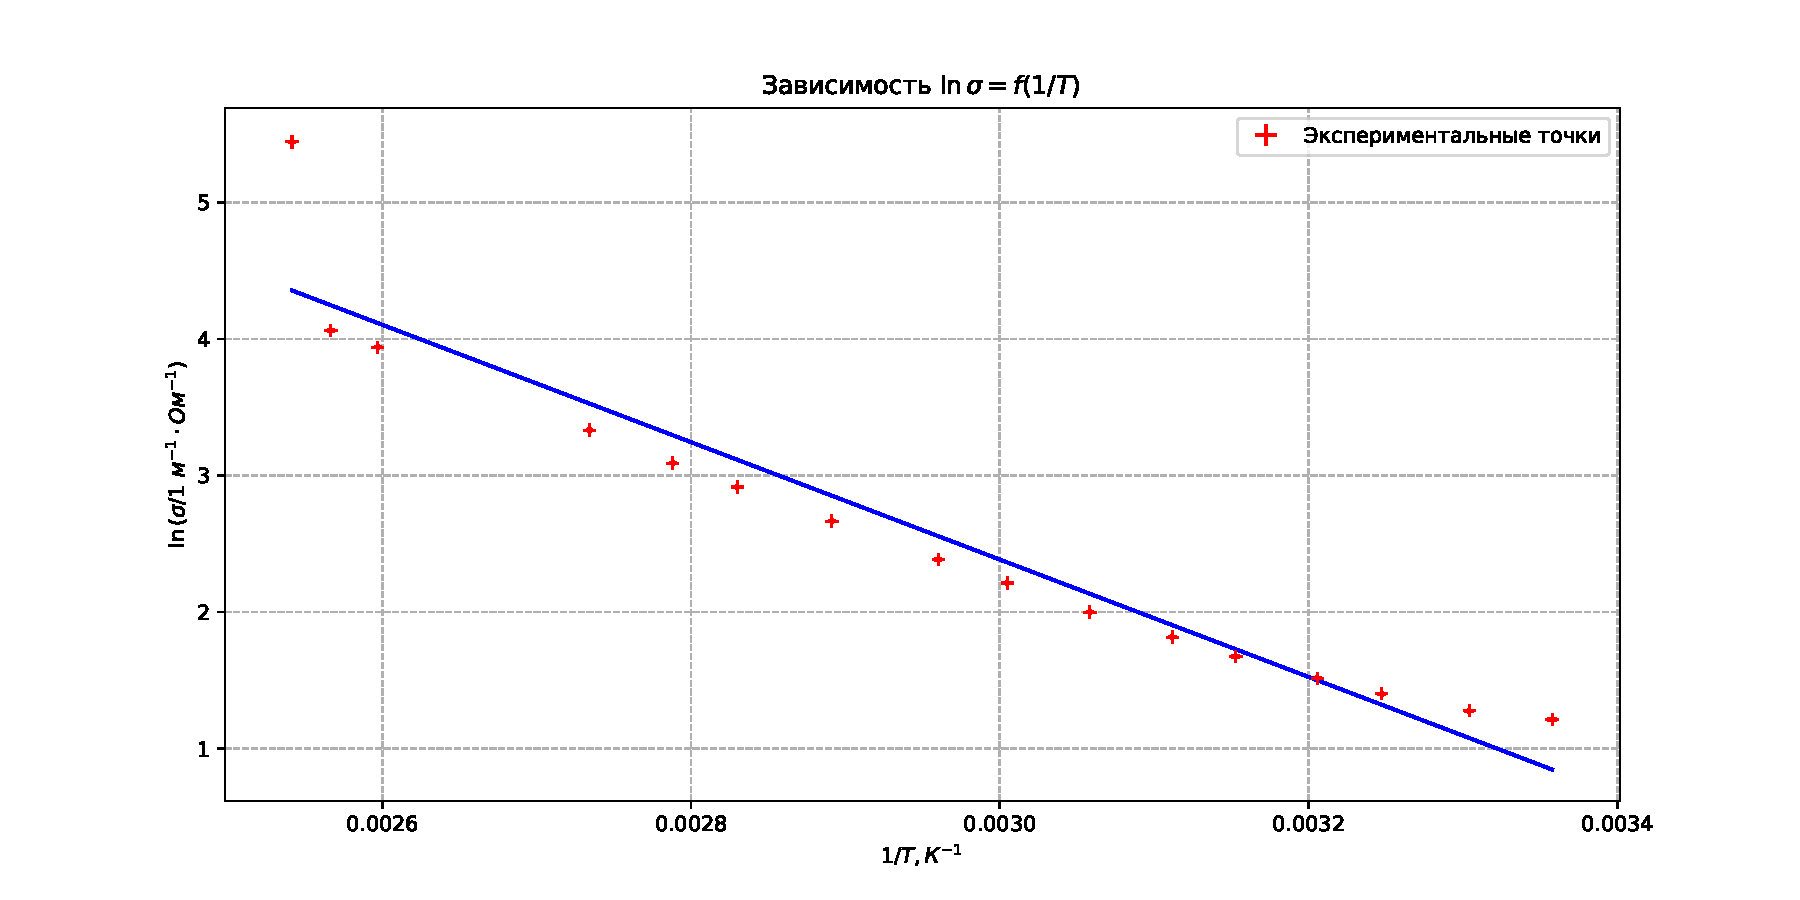
\includegraphics[width=0.9\textwidth]{pictures/ln_sigma_T_graph.pdf}
    \caption{Зависимость $\ln \sigma$ от $1/T$}
    \label{pic:ln-sigma-T}
\end{figure}

В результате линейной аппроксимации получено:

\begin{equation}
    \ln \sigma = (15.3 \pm 1.0) - \frac{(43 \pm 3)\cdot 10^2~\text{К}}{T}.
\end{equation}

По формуле \eqref{eq:delta} получаем

\begin{equation}
    \Delta = (11862 \pm 925)\cdot 10^{-23}~\text{Дж}.
\end{equation}

В электрон-вольтах:

\begin{equation}
    \Delta = (0.74 \pm 0.06)~\text{эВ}.
\end{equation}

\FloatBarrier
\section{Вывод}

\begin{itemize}
    \item Выполнена часть работы с мостом переменного тока: измерена температурная зависимость сопротивления полупроводникового образца и рассчитана электропроводность.

    \item Построены зависимости $\sigma(T)$ и $\ln \sigma(1/T)$. В исследованном диапазоне температур электропроводность возрастает при нагреве, что соответствует полупроводниковому характеру проводимости.

    \item По наклону графика $\ln \sigma(1/T)$ получена ширина запрещённой зоны
    \[
        \Delta = (0.74 \pm 0.06)~\text{эВ}.
    \]
    Полученное значение по порядку величины соответствует германию.
\end{itemize}

\end{document}
